
%% Support sites:
%% http://www.michaelshell.org/tex/ieeetran/
%% http://www.ctan.org/tex-archive/macros/latex/contrib/IEEEtran/
%% and
%% http://www.ieee.org/

%%*************************************************************************
%% Legal Notice:
%% This code is offered as-is without any warranty either expressed or
%% implied; without even the implied warranty of MERCHANTABILITY or
%% FITNESS FOR A PARTICULAR PURPOSE! 
%% User assumes all risk.
%% In no event shall IEEE or any contributor to this code be liable for
%% any damages or losses, including, but not limited to, incidental,
%% consequential, or any other damages, resulting from the use or misuse
%% of any information contained here.
%%
%% All comments are the opinions of their respective authors and are not
%% necessarily endorsed by the IEEE.
%%
%% This work is distributed under the LaTeX Project Public License (LPPL)
%% ( http://www.latex-project.org/ ) version 1.3, and may be freely used,
%% distributed and modified. A copy of the LPPL, version 1.3, is included
%% in the base LaTeX documentation of all distributions of LaTeX released
%% 2003/12/01 or later.
%% Retain all contribution notices and credits.
%% ** Modified files should be clearly indicated as such, including  **
%% ** renaming them and changing author support contact information. **
%%
%% File list of work: IEEEtran.cls, IEEEtran_HOWTO.pdf, bare_adv.tex,
%%                    bare_conf.tex, bare_jrnl.tex, bare_jrnl_compsoc.tex
%%*************************************************************************

% *** Authors should verify (and, if needed, correct) their LaTeX system  ***
% *** with the testflow diagnostic prior to trusting their LaTeX platform ***
% *** with production work. IEEE's font choices can trigger bugs that do  ***
% *** not appear when using other class files.                            ***
% The testflow support page is at:
% http://www.michaelshell.org/tex/testflow/



% Note that the a4paper option is mainly intended so that authors in
% countries using A4 can easily print to A4 and see how their papers will
% look in print - the typesetting of the document will not typically be
% affected with changes in paper size (but the bottom and side margins will).
% Use the testflow package mentioned above to verify correct handling of
% both paper sizes by the user's LaTeX system.
%
% Also note that the "draftcls" or "draftclsnofoot", not "draft", option
% should be used if it is desired that the figures are to be displayed in
% draft mode.
%
\documentclass[conference]{IEEEtran}
% If IEEEtran.cls has not been installed into the LaTeX system files,
% manually specify the path to it like:
% \documentclass[conference]{../sty/IEEEtran}





% Some very useful LaTeX packages include:
% (uncomment the ones you want to load)



% *** CITATION PACKAGES ***
%
\usepackage{cite}
% cite.sty was written by Donald Arseneau
% V1.6 and later of IEEEtran pre-defines the format of the cite.sty package
% \cite{} output to follow that of IEEE. Loading the cite package will
% result in citation numbers being automatically sorted and properly
% "compressed/ranged". e.g., [1], [9], [2], [7], [5], [6] without using
% cite.sty will become [1], [2], [5]--[7], [9] using cite.sty. cite.sty's
% \cite will automatically add leading space, if needed. Use cite.sty's
% noadjust option (cite.sty V3.8 and later) if you want to turn this off.
% cite.sty is already installed on most LaTeX systems. Be sure and use
% version 4.0 (2003-05-27) and later if using hyperref.sty. cite.sty does
% not currently provide for hyperlinked citations.
% The latest version can be obtained at:
% http://www.ctan.org/tex-archive/macros/latex/contrib/cite/
% The documentation is contained in the cite.sty file itself.






% *** GRAPHICS RELATED PACKAGES ***
%
\ifCLASSINFOpdf
   \usepackage[pdftex]{graphicx}
  % declare the path(s) where your graphic files are
  % \graphicspath{{../pdf/}{../jpeg/}}
  % and their extensions so you won't have to specify these with
  % every instance of \includegraphics
  % \DeclareGraphicsExtensions{.pdf,.jpeg,.png}
\else
  % or other class option (dvipsone, dvipdf, if not using dvips). graphicx
  % will default to the driver specified in the system graphics.cfg if no
  % driver is specified.
  % \usepackage[dvips]{graphicx}
  % declare the path(s) where your graphic files are
  % \graphicspath{{../eps/}}
  % and their extensions so you won't have to specify these with
  % every instance of \includegraphics
  % \DeclareGraphicsExtensions{.eps}
\fi
% graphicx was written by David Carlisle and Sebastian Rahtz. It is
% required if you want graphics, photos, etc. graphicx.sty is already
% installed on most LaTeX systems. The latest version and documentation can
% be obtained at: 
% http://www.ctan.org/tex-archive/macros/latex/required/graphics/
% Another good source of documentation is "Using Imported Graphics in
% LaTeX2e" by Keith Reckdahl which can be found as epslatex.ps or
% epslatex.pdf at: http://www.ctan.org/tex-archive/info/
%
% latex, and pdflatex in dvi mode, support graphics in encapsulated
% postscript (.eps) format. pdflatex in pdf mode supports graphics
% in .pdf, .jpeg, .png and .mps (metapost) formats. Users should ensure
% that all non-photo figures use a vector format (.eps, .pdf, .mps) and
% not a bitmapped formats (.jpeg, .png). IEEE frowns on bitmapped formats
% which can result in "jaggedy"/blurry rendering of lines and letters as
% well as large increases in file sizes.
%
% You can find documentation about the pdfTeX application at:
% http://www.tug.org/applications/pdftex





% *** MATH PACKAGES ***
%
%\usepackage[cmex10]{amsmath}
% A popular package from the American Mathematical Society that provides
% many useful and powerful commands for dealing with mathematics. If using
% it, be sure to load this package with the cmex10 option to ensure that
% only type 1 fonts will utilized at all point sizes. Without this option,
% it is possible that some math symbols, particularly those within
% footnotes, will be rendered in bitmap form which will result in a
% document that can not be IEEE Xplore compliant!
%
% Also, note that the amsmath package sets \interdisplaylinepenalty to 10000
% thus preventing page breaks from occurring within multiline equations. Use:
%\interdisplaylinepenalty=2500
% after loading amsmath to restore such page breaks as IEEEtran.cls normally
% does. amsmath.sty is already installed on most LaTeX systems. The latest
% version and documentation can be obtained at:
% http://www.ctan.org/tex-archive/macros/latex/required/amslatex/math/





% *** SPECIALIZED LIST PACKAGES ***
%
\usepackage{algorithm2e}
% algorithmic.sty was written by Peter Williams and Rogerio Brito.
% This package provides an algorithmic environment fo describing algorithms.
% You can use the algorithmic environment in-text or within a figure
% environment to provide for a floating algorithm. Do NOT use the algorithm
% floating environment provided by algorithm.sty (by the same authors) or
% algorithm2e.sty (by Christophe Fiorio) as IEEE does not use dedicated
% algorithm float types and packages that provide these will not provide
% correct IEEE style captions. The latest version and documentation of
% algorithmic.sty can be obtained at:
% http://www.ctan.org/tex-archive/macros/latex/contrib/algorithms/
% There is also a support site at:
% http://algorithms.berlios.de/index.html
% Also of interest may be the (relatively newer and more customizable)
% algorithmicx.sty package by Szasz Janos:
% http://www.ctan.org/tex-archive/macros/latex/contrib/algorithmicx/





% *** ALIGNMENT PACKAGES ***
%
%\usepackage{array}
% Frank Mittelbach's and David Carlisle's array.sty patches and improves
% the standard LaTeX2e array and tabular environments to provide better
% appearance and additional user controls. As the default LaTeX2e table
% generation code is lacking to the point of almost being broken with
% respect to the quality of the end results, all users are strongly
% advised to use an enhanced (at the very least that provided by array.sty)
% set of table tools. array.sty is already installed on most systems. The
% latest version and documentation can be obtained at:
% http://www.ctan.org/tex-archive/macros/latex/required/tools/


%\usepackage{mdwmath}
%\usepackage{mdwtab}
% Also highly recommended is Mark Wooding's extremely powerful MDW tools,
% especially mdwmath.sty and mdwtab.sty which are used to format equations
% and tables, respectively. The MDWtools set is already installed on most
% LaTeX systems. The lastest version and documentation is available at:
% http://www.ctan.org/tex-archive/macros/latex/contrib/mdwtools/


% IEEEtran contains the IEEEeqnarray family of commands that can be used to
% generate multiline equations as well as matrices, tables, etc., of high
% quality.


%\usepackage{eqparbox}
% Also of notable interest is Scott Pakin's eqparbox package for creating
% (automatically sized) equal width boxes - aka "natural width parboxes".
% Available at:
% http://www.ctan.org/tex-archive/macros/latex/contrib/eqparbox/





% *** SUBFIGURE PACKAGES ***
\usepackage[tight,footnotesize]{subfigure}
% subfigure.sty was written by Steven Douglas Cochran. This package makes it
% easy to put subfigures in your figures. e.g., "Figure 1a and 1b". For IEEE
% work, it is a good idea to load it with the tight package option to reduce
% the amount of white space around the subfigures. subfigure.sty is already
% installed on most LaTeX systems. The latest version and documentation can
% be obtained at:
% http://www.ctan.org/tex-archive/obsolete/macros/latex/contrib/subfigure/
% subfigure.sty has been superceeded by subfig.sty.



%\usepackage[caption=false]{caption}
%\usepackage[font=footnotesize]{subfig}
% subfig.sty, also written by Steven Douglas Cochran, is the modern
% replacement for subfigure.sty. However, subfig.sty requires and
% automatically loads Axel Sommerfeldt's caption.sty which will override
% IEEEtran.cls handling of captions and this will result in nonIEEE style
% figure/table captions. To prevent this problem, be sure and preload
% caption.sty with its "caption=false" package option. This is will preserve
% IEEEtran.cls handing of captions. Version 1.3 (2005/06/28) and later 
% (recommended due to many improvements over 1.2) of subfig.sty supports
% the caption=false option directly:
%\usepackage[caption=false,font=footnotesize]{subfig}
%
% The latest version and documentation can be obtained at:
% http://www.ctan.org/tex-archive/macros/latex/contrib/subfig/
% The latest version and documentation of caption.sty can be obtained at:
% http://www.ctan.org/tex-archive/macros/latex/contrib/caption/




% *** FLOAT PACKAGES ***
%
%\usepackage{fixltx2e}
% fixltx2e, the successor to the earlier fix2col.sty, was written by
% Frank Mittelbach and David Carlisle. This package corrects a few problems
% in the LaTeX2e kernel, the most notable of which is that in current
% LaTeX2e releases, the ordering of single and double column floats is not
% guaranteed to be preserved. Thus, an unpatched LaTeX2e can allow a
% single column figure to be placed prior to an earlier double column
% figure. The latest version and documentation can be found at:
% http://www.ctan.org/tex-archive/macros/latex/base/



%\usepackage{stfloats}
% stfloats.sty was written by Sigitas Tolusis. This package gives LaTeX2e
% the ability to do double column floats at the bottom of the page as well
% as the top. (e.g., "\begin{figure*}[!b]" is not normally possible in
% LaTeX2e). It also provides a command:
%\fnbelowfloat
% to enable the placement of footnotes below bottom floats (the standard
% LaTeX2e kernel puts them above bottom floats). This is an invasive package
% which rewrites many portions of the LaTeX2e float routines. It may not work
% with other packages that modify the LaTeX2e float routines. The latest
% version and documentation can be obtained at:
% http://www.ctan.org/tex-archive/macros/latex/contrib/sttools/
% Documentation is contained in the stfloats.sty comments as well as in the
% presfull.pdf file. Do not use the stfloats baselinefloat ability as IEEE
% does not allow \baselineskip to stretch. Authors submitting work to the
% IEEE should note that IEEE rarely uses double column equations and
% that authors should try to avoid such use. Do not be tempted to use the
% cuted.sty or midfloat.sty packages (also by Sigitas Tolusis) as IEEE does
% not format its papers in such ways.





% *** PDF, URL AND HYPERLINK PACKAGES ***
%
%\usepackage{url}
% url.sty was written by Donald Arseneau. It provides better support for
% handling and breaking URLs. url.sty is already installed on most LaTeX
% systems. The latest version can be obtained at:
% http://www.ctan.org/tex-archive/macros/latex/contrib/misc/
% Read the url.sty source comments for usage information. Basically,
% \url{my_url_here}.





% *** Do not adjust lengths that control margins, column widths, etc. ***
% *** Do not use packages that alter fonts (such as pslatex).         ***
% There should be no need to do such things with IEEEtran.cls V1.6 and later.
% (Unless specifically asked to do so by the journal or conference you plan
% to submit to, of course. )


% correct bad hyphenation here
\hyphenation{op-tical net-works semi-conduc-tor}


\begin{document}
%
% paper title
% can use linebreaks \\ within to get better formatting as desired
\title{Jaguar Lite Point Tracking}

\author{\IEEEauthorblockN{Lauren Lieu}
\IEEEauthorblockA{
Department of Engineering\\
Harvey Mudd College\\
Email: llieu@g.hmc.edu}
\and
\IEEEauthorblockN{Joshua Vasquez}
\IEEEauthorblockA{Department of Engineering\\
Harvey Mudd College\\
Email: jvasquez@g.hmc.edu}
}

% make the title area
\maketitle
{\flushleft March 5, 2013}\\
\IEEEpeerreviewmaketitle

\begin{abstract}
This paper describes the implementation of point tracking for the \emph{Jaguar Lite Mobile Robot Platform}. Motion control of the autonomous vehicle is achieved using a Proportional-Integral-Derivative controller. In both simulation and hardware mode, the control law parameters and control gains have been tuned to demonstrate stable, precise motion towards desired goal poses.
\end{abstract} 

\section{Introduction}
\emph{Point Tracking} refers to a robot's ability to transition 
from one pose to another on a known map of its environment. By modeling the 
robot's drive train with a motion model and by incorporating odometric 
sensor readings into this motion model, the robot can develop a trajectory 
between points.  In the following paper, we incorporate both a differential drive-train 
motion model with a PID-controlled differential drive train to designate the
Jaguar Lite robotic platform to track points on a two-dimensional environment.

\subsection{Hardware Platform}
The hardware platform of choice is a Jaguar Lite autonomous vehicle, sourced 
by Dr. Robot.  This differential-drive platform is fairly rugged, and 
features a suite of sensory inputs: a 9 DOF Inertial measurement unit (IMU), 
two rotary encoders, a 240$^{\circ}$ field-of-view laser range finder, and an
onboard webcam \cite{Dr.RobotWebsite}.  With a wireless wifi interface, the 
designer can implement navigation algorithms in \emph{C\#} within Microsoft Visual Studio to communicate with the Jaguar platform. Most importantly, the platform can  be driven both 
indoors and outdoors. 

\begin{figure}[h]
\centering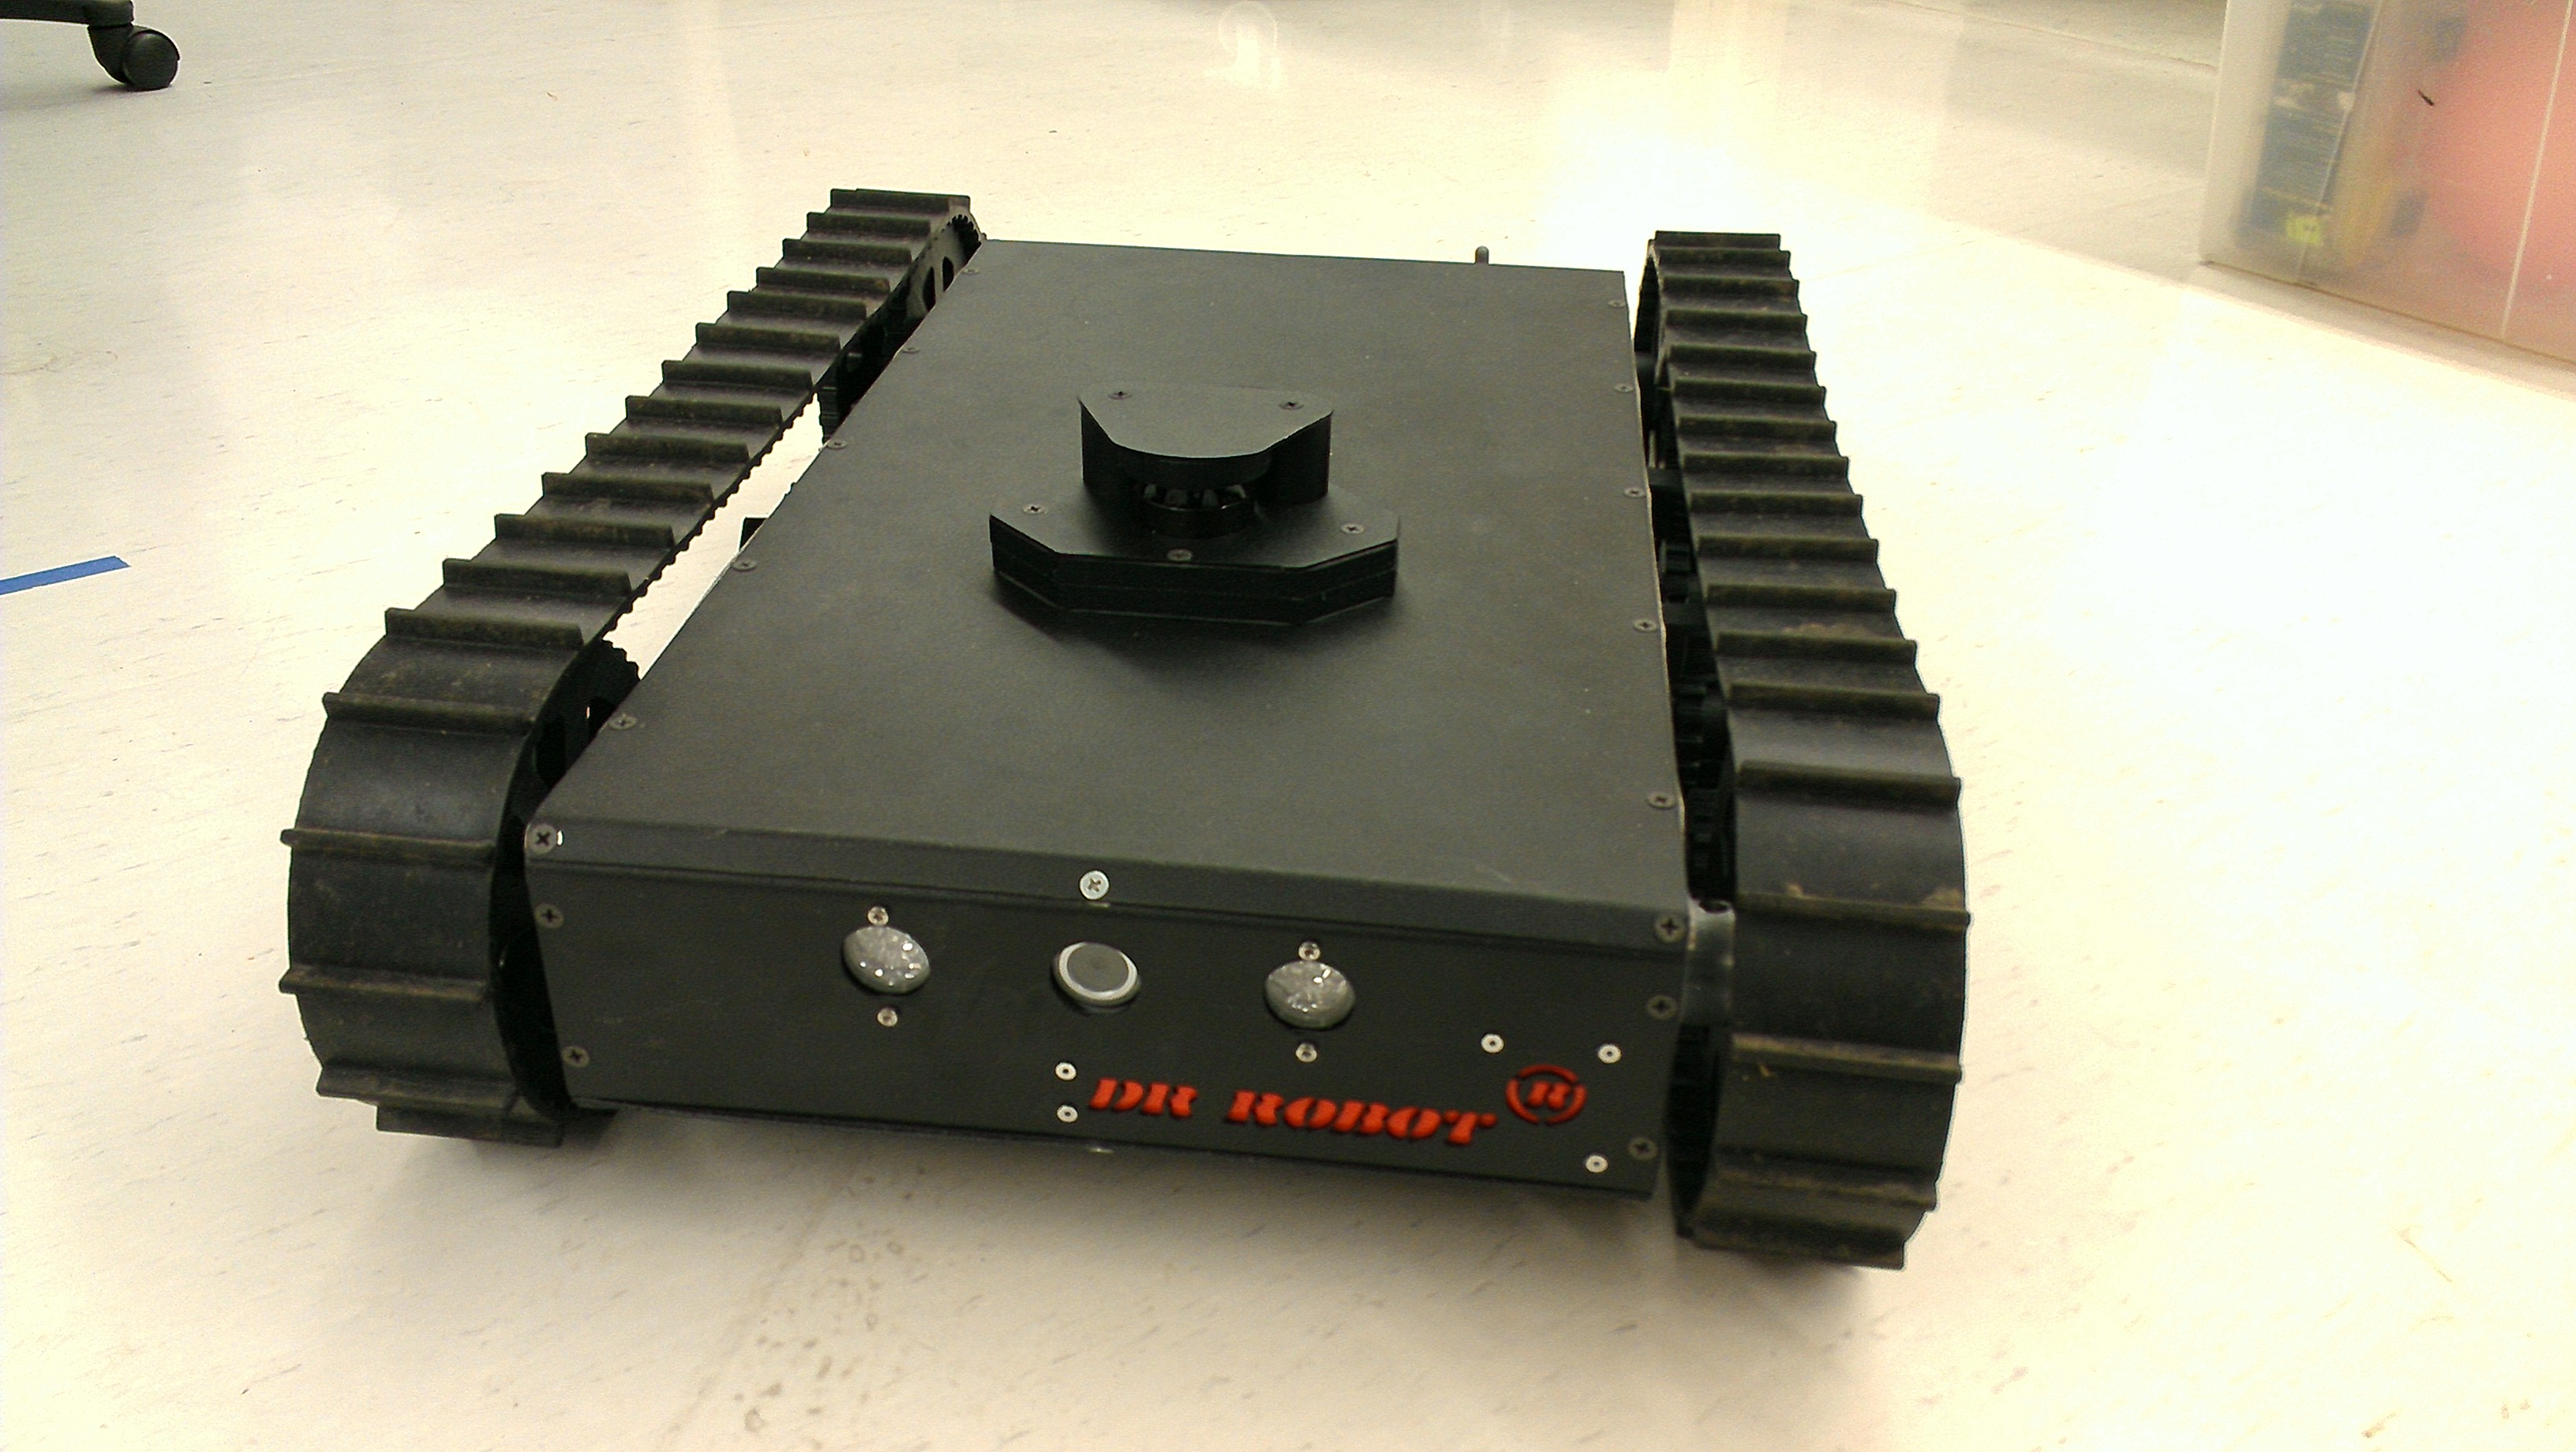
\includegraphics[width = 3in]{jaguarLite.png}
\caption{The Jaguar Lite Platform}
\label{fig1}
\end{figure}

\subsection{Terminology}
This paper refers to specific definitions and usage of the following terms:

\begin{itemize}
\item \noindent \textbf{Pose} represents the robot's position: $[x,y,\theta]$ relative to a 
coordinate frame fixed to the environment that the robot navigates.
 
\item \noindent \textbf{Nonholonomic Constraints} refers to a restricted motion path 
constrained by the physcial construction of the robot.  On a two-dimensional coordinate 
frame, a robot that can freely
rotate and translate is considered a holonomic robot. 

\item \noindent \textbf{Point Tracking} refers to the Jaguar Lite's ability to drive
from one pose to another on a navigable coordinate frame.

\end{itemize}
\section{Background}
\section{Problem Definition}
\section{Control Design}

\subsection{Motion Model}
Developing a method of navigating from one pose to another simplifies to determining 
the appropriate motor speeds of the Jaguar Lite at any given pose to form a trajectory as the robot pursues a goal pose.  
To determine the robot's motor outputs, an effective motion model which reflects
the robot's nonholonomic constraints must be used. 

\begin{figure}[!h]
\centering
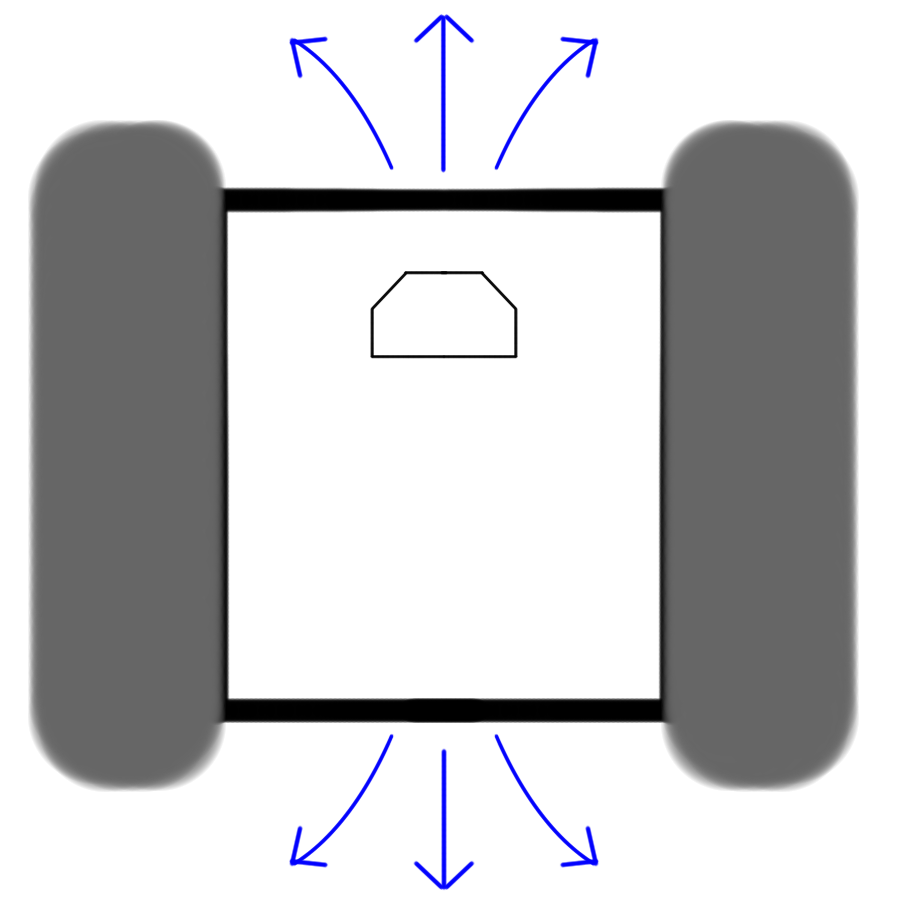
\includegraphics[width =2in]{pic1.png}
\caption{Realizable Trajectories}
\label{fig2}
\end{figure}

The Jaguar Lite moves with a differential drive train.  For this reason, the motion model cannot 
incorporate direct translation of the robot in a direction normal to the sides of
the robot. Figure~\ref{fig2} illustrates possible trajectories, each of which is 
governed by the speed of the right wheel $\omega_1$ and the left wheel $\omega_2$.

%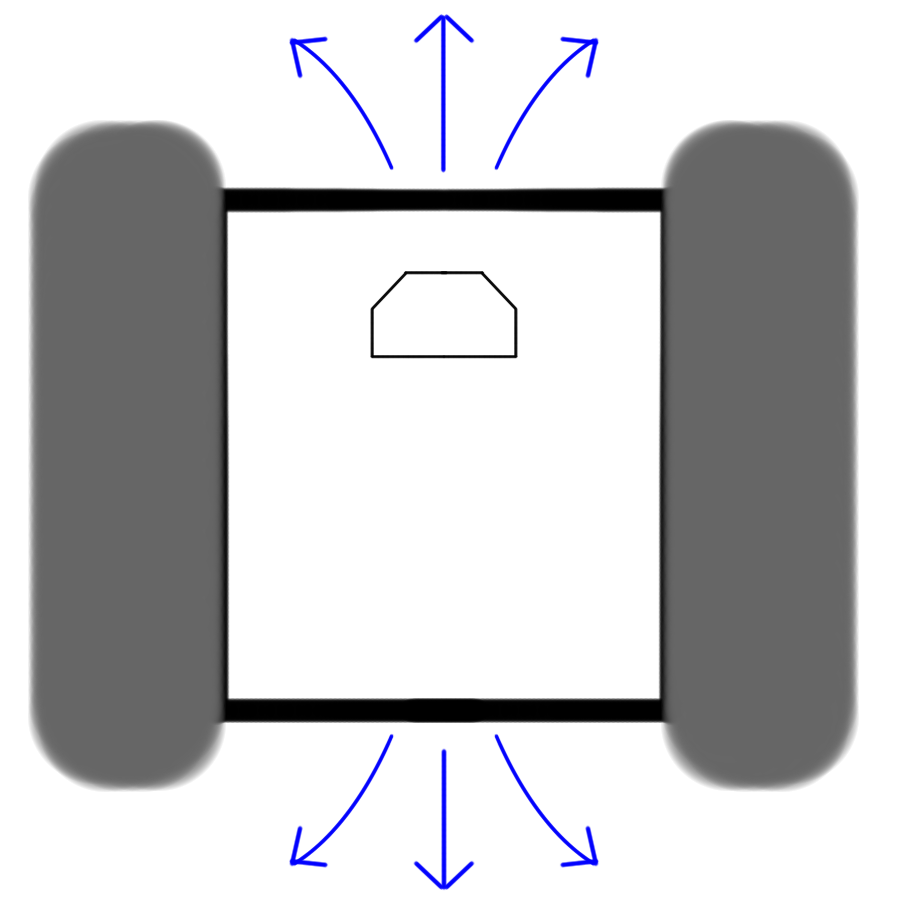
\includegraphics[width =2.5in]{pic1.png}
%\textbf{Figure 2. Realizable Trajectories}

Given a differential drive train, we can use the following coordinate transform 
to describe the robot's pose relative to the goal pose \cite{Textbook}:

\begin{equation} \label{eq:rho}
\rho = \sqrt{\Delta x^2 + \Delta y^2}
\end{equation}
\begin{equation} \label{eq:alpha}
\alpha = -\theta + atan2(\Delta y, \Delta x)
\end{equation}
\begin{equation} \label{eq:beta}
\beta = -\theta -\alpha
\end{equation}

Equations (\ref{eq:rho}), (\ref{eq:alpha}), and (\ref{eq:beta}) $x$ and $y$ define the horizontal and vertical displacements
respectively, relative to a fixed global coordinate frame.  $\theta$ defines the 
angular displacement of the robot normal vector relative to the x axis.  
$\rho$ defines the magnitude of the displacement from the robot's pose to the 
goal pose.  $\alpha$ defines the error of the robot normal vector relative to 
the desired angle relative to the goal.  $\beta$ defines the angle of the goal vector 
relative to the horizontal.  The angles of the coordinate transformation are shown in Figure~\ref{fig3}. 

\begin{figure}
\centering
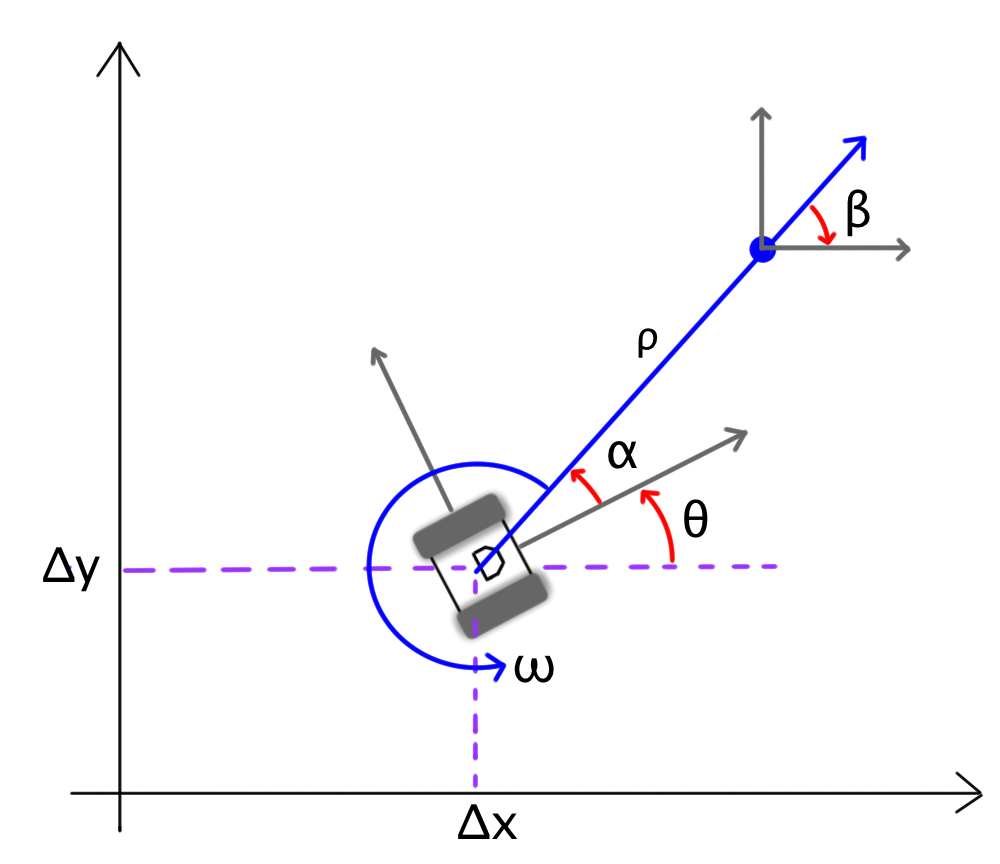
\includegraphics[width = 3in]{pic2.png}
\caption{Linear and Angular Errors}
\label{fig3}
\end{figure}

The above equations quantify the error, or difference between the robot's pose and
the desired pose.  By calculating the kinematics in this coordinate frame and applying the control law, equations (\ref{eq:vel}) and (\ref{eq:omega}) can be produced, which define the
Jaguar Lite's linear velocity $v$ and angular velocity $\omega$ as a 
function of the error values $\rho$, $\alpha$, and $\beta$.  

\begin{equation}\label{eq:vel}
v = k_{\rho} \rho
\end{equation}
\begin{equation}\label{eq:omega}
\omega = k_{\alpha} \alpha  +  k_{\beta} \beta 
\end{equation}
where $k_{\rho}$, $k_{\alpha}$, and $k_{\beta}$ are tuned gain constants.

Given that equations  (\ref{eq:vel}) and (\ref{eq:omega}) model the robot's desired
 change in displacement over time, this motion control must be achieved on the Jaguar Lite platform
through control of the left and right wheel rotations.  Equations (\ref{eq:wheel1}) and (\ref{eq:wheel2}) fulfill 
this requirement.
\begin{equation}\label{eq:wheel1}
\omega(t) = \omega_1 + \omega_2 
\end{equation} 
\begin{equation}\label{eq:wheel2}
v(t) = L \left( \omega_1 - \omega_2 \right)
\end{equation}
where $L$ is the radius of the robot.
Thus, the overall left and right angular velocities, $\omega_1$ and $\omega_2$ respectively, may 
be determined by combining the previous equations to produce:
\begin{equation}
\omega_1 = \frac{v}{2L} + \frac{\omega}{2}
\end{equation}

\begin{equation}
\omega_2 = -\frac{v}{2L} + \frac{\omega}{2} 
\end{equation}

\subsection{PID Motor Control}
The above equations rely on accurate determination and control of the left and right
wheel speeds.  To determine the actual wheel speeds the Jaguar Lite receives 
sensory input from quadrature encoders. 
Overall, the point tracking trajectory becomes far more accurate in implementation
if the left and right motor speeds are controlled with a tight control loop.
Thus, the desired left and right motor speeds (derived from $\omega_1$ and $\omega_2$)
can be far more closely approximated by the actual Jaguar hardware.
To achieve wheel-speed control, a PID controller was implemented
to stabilize the individual wheel speeds of both motors.

At the lower level the Jaguar Lite's left and right wheel motors can 
change speed through pulse-width modulation, and a specified 
duty cycle.  By tuning the $P$, $I$, and $D$ control gains, the controller changes the 
duty cycle, effectively maintaining  
wheel velocities far closer to the desired values.

%% not sure if this still jives with the rest
%Assuming the robot is travelling on a circular arc of constant radius, we can apply basic circle geometry to calculate the distance traveled $\Delta s$ and the change in orientation $\Delta\theta$ of each tread of the Jaguar Lite robot for time step $\Delta t$. These changes in displacement are within the local coordinate frame of the robot. To convert the position change of the robot into the global coordinate frame, we assume that the robot's motion is small in a given time step. As a result, the robot's trajectory can be approximated to be a straight path, and using trigonometry we derived the following equations to determine the change in position within a global coordinate frame, where $L$ is the radius of the robot.

\section{Results}

The three control gains $K_{\rho}$ $K_{\alpha}$, and $K_{\beta}$ weight the influence 
of each error parameter, iterating through time to measure the displacement of the robot
relative to the goal pose. By tuning these parameters both in simulation and hardware modes, 
the desired correction velocities were achieved. In simulation, the tuned parameter values are 
$K_{\rho} = 1$ $K_{\alpha} =  3$, and $K_{\beta} = -2$ while in hardware the optimal values 
are $K_{\rho} = 4$ $K_{\alpha} =  4.5$, and $K_{\beta} = -4.5$.

\begin{figure}[b]
\centering
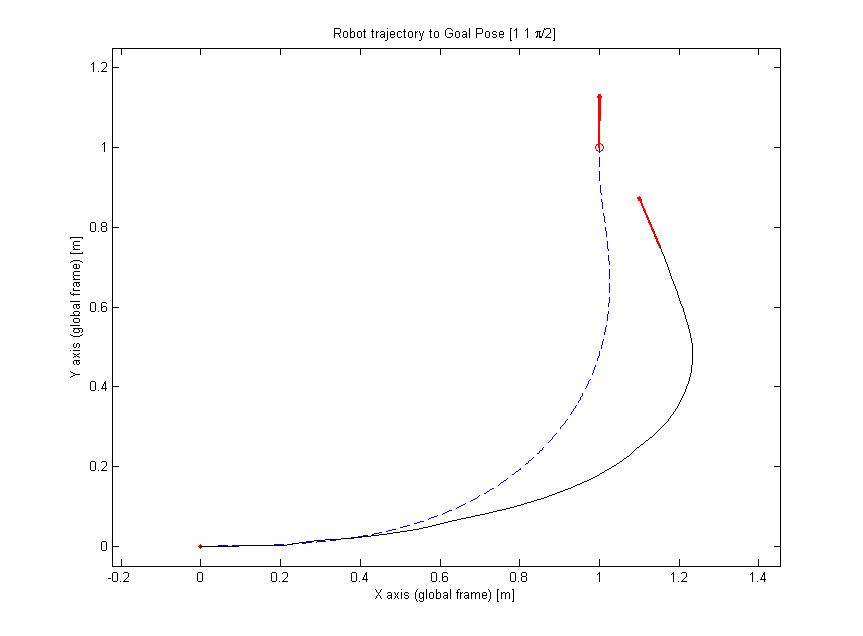
\includegraphics[width = 3.5in]{trajectory.jpg}
\caption{Simulated robot trajectory (blue, dashed) and actual Jaguar Lite trajectory (black) with final poses (red).}
\label{fig4}
\end{figure}

For experimental testing, tuning the three $P$, $I$, $D$
controller constants of the motor velocity controller also guided the Jaguar Lite to its goal pose. 
With the tuned control gains $P = 14$, $I = 5$ and $D = 12$ the robot successfully traverses from an initial pose at the origin to a goal pose within range of the 
actual desired final point. The trajectory of the robot in simulation and hardware is shown in Figure ~\ref{fig4}.

The presented motion model and control law does not encompass all cases of possible robot 
locomotion. In particular, this control design does not account for spinning the robot in place at a 
given pose when $x$ and $y$ remain fixed.  This arises when the robot is already at the location 
of its goal pose, such that $\rho$ is zero, but its orientation $\theta$ is different angle than the desired angle.  Given the 
Jaguar Lite's ability to spin in place, this possibile method of movement is not encompassed by equations
 (\ref{eq:rho}), (\ref{eq:alpha}), and (\ref{eq:beta}).  
However, by removing the $\alpha$ term in equation (\ref{eq:alpha}), corrected desired velocities 
can be written as follows:
\begin{equation} 
v = 0
\end{equation}
\begin{equation}
\omega = K_{\beta} \beta 
\end{equation}

Thus, redefining $v$ and $\omega$ when $\rho$ is sufficiently small allows the robot to rotate 
in place. The hardware implementation of this type of locomotion is limited depending on the 
terrain, however, simulation testing of this control design was successful.


\section{Conclusion}
By implementing this control design and combining this with odometry-based localization, the Jaguar 
Lite can effectively traverse from one pose to a set goal pose.
Furthermore, by simplifing trajectories into a series of desired poses,
point tracking presents a powerful solution to generating trajectories 
for the robot to follow.  Thus, the initial development of a motion model
can effectively lead to the implementation of obstacle avoidance, 
tracking of waypoints and continuous path following on a known map.

Future work 
includes extending and applying point tracking capabilities to track 
straight and curved trajectories, and also incorporating odometry error 
characterization to correct for the drift identified in the Jaguar Lite encoder hardware.


\section*{Acknowledgment}


The authors would like to thank Professor Christopher Clark for 
establishing a software framework for algorithm development and
 providing hardware resources from the Lab for Autonomous and
 Intelligent Robotics.




\begin{thebibliography}{1}

\bibitem{LaboratoryExercise1}%IEEEhowto:kopka}
\begin{verbatim}
http://newwww.hmc.edu/lair/E190Q/
E190Q-Lab01-IntroToTheJaguar.pdf
\end{verbatim}

\bibitem{Dr.RobotWebsite}
\begin{verbatim}
http://jaguar.drrobot.com/specification_lite.asp
\end{verbatim}

\bibitem{PDFOfEquations}
\begin{verbatim}
http://newwww.hmc.edu/lair/E190Q/
E190Q-Lecture04-PointTracking.pdf
\end{verbatim}

\bibitem{Textbook}
Siegwart Roland, et al. \emph{Introduction to Autonomous Mobile Robots} 2nd ed. 
2011 MIT Press

\bibitem{Probabilistic}
Thrun, Sebastian, et. all. \emph{Probabilistic Robotics}
2005, The MIT Press.


\end{thebibliography}




% that's it, dude!
\end{document}


